\begin{table}[H]
    {\renewcommand{\arraystretch}{1.2}%
    \setlength{\tabcolsep}{0.6em}%
    \footnotesize
\begin{tabular}{bababab}
\toprule

\rowcolor{white} \null &
\textbf{Synthetic$_{\mathbf{\mathcal{F}}}$} & \textbf{Synthetic$_{\mathbf{\mathcal{\beta}}}$} &
\textbf{Lehrpfad$_{\mathbf{\mathcal{F}}}$} & \textbf{Lehrpfad$_{\mathbf{\mathcal{\beta}}}$} &
\textbf{Office$_{\mathbf{\mathcal{F}}}$} & \textbf{Office$_{\mathbf{\mathcal{\beta}}}$} \\
\midrule

\rowcolor{lightgray}
\textbf{Keypoint Count} &
    \num{217505} & \num{44221} &
    \num{2168190} & \num{2198592} &
    \num{171000} & \num{171000} \\
\textbf{Correspondences} &
    \num{96371} & \num{26455} &
    \num{297949} & \num{222495} &
    \num{43037} & \num{36309} \\
\rowcolor{lightgray}
\textbf{True Positives} &
    \num{76603} & \num{22179} &
    \num{110339} & \num{35387} &
    \num{24025} & \num{15455} \\
\textbf{False Positives} &
    \num{59032} & \num{8865} &
    \num{648603} & \num{651091} &
    \num{48868} & \num{48697} \\
\rowcolor{lightgray}
\textbf{False Negatives} &
    \num{19768} & \num{4276} &
    \num{187610} & \num{187108} &
    \num{19012} & \num{20854} \\

\bottomrule
\end{tabular}

    }
    \caption[Keypoint and matching results for \texttt{\acrshort{akaze}/raw/default}]{\emph{Keypoint and matching results for \texttt{\acrshort{akaze}/raw/default}.} \acrshort{akaze} achieves better results than \acrshort{surf} and \acrshort{orb}. The number of correspondences is very high compared to \acrshort{sift}, but true positives are still higher than false negatives. This indicates reasonable descriptor performance and stability of the keypoint detector.}
\end{table}
The final evaluated feature detection algorithm is \acrshort{akaze}.
Its keypoint detector design is again closer to \acrshort{sift}.
\acrshort{akaze} results in approximately one order of magnitude more detected keypoints and correspondences compared to \acrshort{sift}.
Its keypoint characteristics show expected results (Appendix~\ref{sec:akaze_stats}).
The detection does not result in as similar diverse keypoint sizes and the response is narrower with a stronger skew towards small responses compared to \acrshort{sift}.
\begin{figure}[b!]
\begin{subfigure}[t]{0.45\linewidth}
    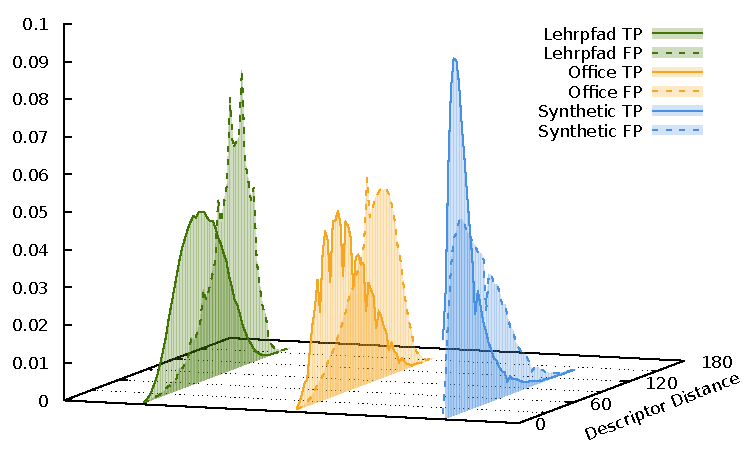
\includegraphics[width=\linewidth]{chapter06/results/AKAZE/flexion/descriptor_distances.pdf}%
    \caption{\glspl{flexion-image}}
\end{subfigure}\quad
\begin{subfigure}[t]{0.45\linewidth}
    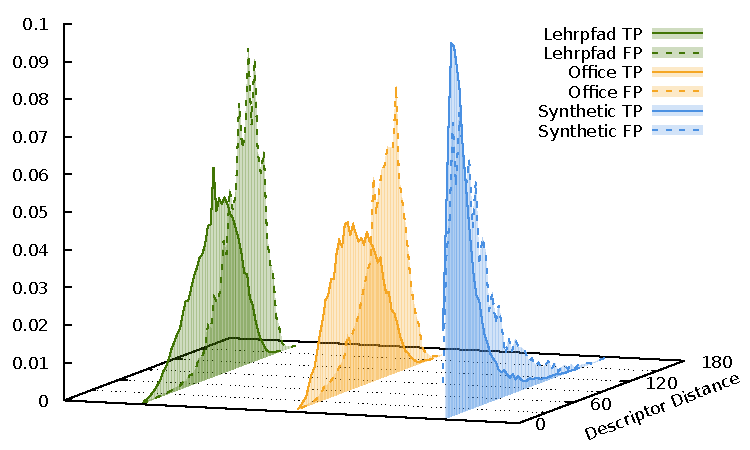
\includegraphics[width=\linewidth]{chapter06/results/AKAZE/bearing/descriptor_distances.pdf}%
    \caption{\glspl{bearing-angle-image}}
\end{subfigure}
\caption[\acrshort{akaze} descriptors distances]{\emph{\acrshort{akaze} descriptors distances.} The true and false positives are partially separable by the descriptor distance. The \gls{flexion-image} shows better separation than the \gls{bearing-angle-image}. The descriptor is binary and similar to \acrshort{orb}'s descriptor, but the improvements show measurable effects.}\label{fig:descriptor_akaze}
\end{figure}
The \acrshort{mldb} descriptor shows separation between true and false positives across the datasets and feature images (Figure~\ref{fig:descriptor_akaze}).
This indicates good performance of the binary descriptor.
Additionally it reaffirms the finding of \acrshort{orb}'s \acrshort{brief} descriptor demonstrating separation potential.
The enhancement of \acrshort{mldb} solidifies the tendency though.
The \acrshort{ROC} graph in Figure~\ref{fig:roc_akaze} shows that \acrshort{akaze} can perform quiet reasonable across all datasets.
There exists a configuration for each dataset with significantly higher true than false positive rate for the \glspl{flexion-image}.
The top performers for each dataset are the configurations using only the best 400 keypoints for matching, regardless of filtering.
Applying additional heuristics in matching, like a maximum matching distance, will certainly improve the ratio of true to false positives further.
The backprojections in Appendix~\ref{sec:backprojection_akaze} show the higher amount of keypoints compared to \acrshort{sift}.
But bad scale coverage leads to unsatisfying keypoint coverage for the \emph{Laserscan} dataset.
There, \acrshort{sift} has clear qualitative advantages over \acrshort{akaze}, because its keypoints cover the whole scan.
\begin{figure}[H]
\begin{subfigure}[t]{0.45\linewidth}
    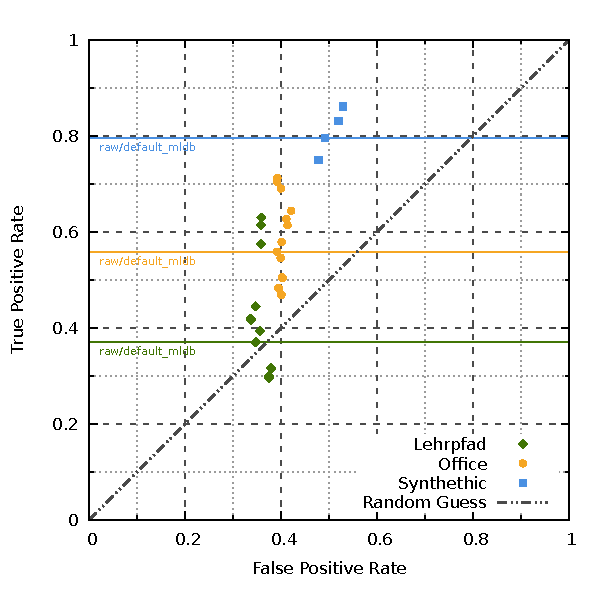
\includegraphics[width=\linewidth]{chapter06/results/AKAZE/flexion/roc.pdf}%
    \caption{\gls{flexion-image}}
\end{subfigure}\quad
\begin{subfigure}[t]{0.45\linewidth}
    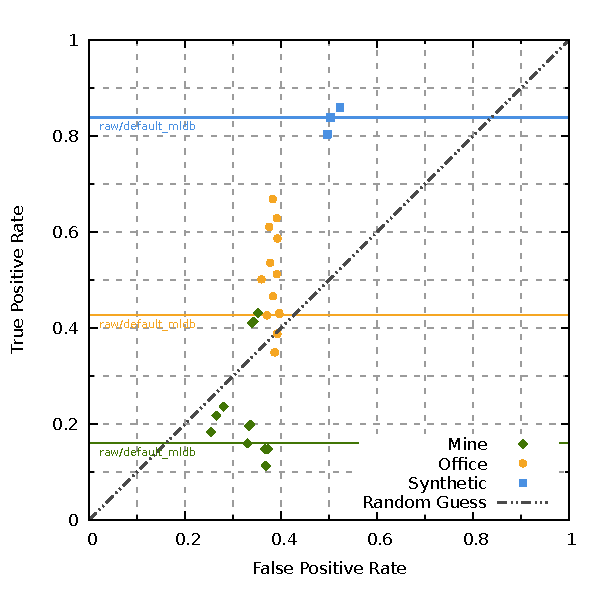
\includegraphics[width=\linewidth]{chapter06/results/AKAZE/bearing/roc.pdf}
    \caption{\gls{bearing-angle-image}}
\end{subfigure}
    \caption[\acrshort{ROC} graphs for \acrshort{akaze}]{\emph{\acrshort{ROC} graphs for \acrshort{akaze}.} \acrshort{akaze} results in a bigger spread of the algorithm performance depending on the configuration. The \gls{bearing-angle-image} falls behind the \gls{flexion-image}. The higher scoring configurations apply filtering of the keypoints by their response.}\label{fig:roc_akaze}
\end{figure}
